%% Author_tex.tex
%% V1.0
%% developed by Nova Techset
%%
%% This file describes the coding for COB.cls

\documentclass[vruler,JEB]{COB}%%%%where COB is the template name

%The authors can define any packages after the \documentclass{COB} command.

%\usepackage{amsmath} for dealing with mathematics,
%\usepackage{amsthm} for dealing with theorem environments,
%\usepackage{cite} for dealing with citations
%\usepackage{hyperref} for linking the cross references
%\usepackage{graphics} for dealing with figures.
%\usepackage{algorithmic} for describing algorithms
%\usepackage{subfig} for getting the subfigures e.g., "Figure 1a and 1b" etc.
%\usepackage{url} It provides better support for handling and breaking URLs.

\usepackage{widetext-TI}

\newtheorem{theorem}{Theorem}
\newtheorem{condition}{Condition}


%The author can find the documentation of the above style file and any additional
%supporting files if required from "http://www.ctan.org"

% *** Do not adjust lengths that control margins, column widths, etc. ***

\begin{document}

\supertitle{Research Article}

\title{How to use the Company of Biologists (\JABBR) \LaTeX\ class}

\author{First author$^{1}$ and Second author$^{2}$}

\address{\add{1}{First author address}
\add{2}{Second author address}}

\corres{(\email{xxxx@xxxx.xxx.xx}; \email{xxxx@xxxx.xxx.xx})}

\date{Received 1 May 2018; revised 5 December 2018}

\maketitle

\begin{abstract}
This sample is a guideline for preparing technical papers
using \LaTeX. It contains the documentation for a \LaTeX\
class file that creates the correct manuscript layout for
any of the Company of Biologists journals: Development,
Journal of Cell Science, Journal of Experimental Biology,
Biology Open or Disease Models and Mechanisms. This sample
file uses a class file named \texttt{COB.cls}, which authors should
use during manuscript preparation.
\end{abstract}

\keywords{keyword entry 1, keyword entry 2, keyword entry~3}


\section{Insert A head here}
This demo file is intended to serve as a ``starter file''
for author manuscripts produced under \LaTeX\ using
COB.cls.

\subsection{Insert B head here}
Subsection text here.


\subsubsection{Insert C head here}
Subsubsection text here.

\section{Spanning equation across two column}

In order to span the equations across two columns, please use the command
\verb+\begin{widetext}...\end{widetext}+ command (see equation 1).

\begin{widetext}
\begin{align} \label{d24} x_{\sigma+1} &= x_{\sigma} + \left( \dfrac{1-\alpha(t_\sigma)}{M[\alpha(t_\sigma)]} + \dfrac{3h\alpha(t_\sigma)}{2M[\alpha(t_\sigma)]} \right)  \left\{-bx(t_\sigma-m_1) + a \sin [cx(t_\sigma-m_2)]\right\}  - \left( \dfrac{1-\alpha(t_\sigma)}{M[\alpha(t_\sigma)]} + \dfrac{h \alpha(t_\sigma)}{2M[\alpha(t_\sigma)]}\right)\nonumber\\ &\quad\times \left\{-bx(t_\sigma-m_1) + a \sin [cx(t_\sigma-m_2)]\right\}. \end{align}
\end{widetext}


\section{Equations}

Sample equations.

%%% Numbered equation
\begin{align}\label{1.1}
\begin{split}
\frac{\partial u(t,x)}{\partial t} = Au(t,x) \left(1-\frac{u(t,x)}{K}\right)\\
\quad -B\frac{u(t-\tau,x) w(t,x)}{1+Eu(t-\tau,x)},\\
\frac{\partial w(t,x)}{\partial t} =\delta \frac{\partial^2w(t,x)}{\partial x^2}-Cw(t,x)\\
+D\frac{u(t-\tau,x)w(t,x)}{1+Eu(t-\tau,x)},
\end{split}
\end{align}


\begin{align}\label{1.2}
\begin{split}
\notag\\[-26pt]\frac{dU}{dt} &=\alpha U(t)(\gamma -U(t))-\frac{U(t-\tau)W(t)}{1+U(t-\tau)},\\
\frac{dW}{dt} &=-W(t)+\beta\frac{U(t-\tau)W(t)}{1+U(t-\tau)}.
\end{split}
\end{align}


%%%% Unnumbered equation
\begin{align*}
&\frac{\partial(F_1,F_2)}{\partial(c,\omega)}_{(c_0,\omega_0)} = \left|
\begin{array}{ll}
\frac{\partial F_1}{\partial c} &\frac{\partial F_1}{\partial \omega} \\\noalign{\vskip3pt}
\frac{\partial F_2}{\partial c}&\frac{\partial F_2}{\partial \omega}
\end{array}\right|_{(c_0,\omega_0)}\\
&\quad=-4c_0q\omega_0 -4c_0\omega_0p^2 =-4c_0\omega_0(q+p^2)>0.
\end{align*}


\section{Enunciations}
%%%% Most of the enunciations like theorem, lemma, corollary, proposition, defintion,
%%%% condition, example, conjecture etc. are defined in the class file.

%%%% If the author wants to add or modify the enunciation style
%%%% they can define in the preamble as shown below.

%%%% \newtheoremstyle{theorem}{6pt}{6pt}{\rm}{}{\sffamily}{ }{ }{}
%%%% \theoremstyle{theorem}
%%%% \newtheorem{theorem}{\sc Theorem}[section]

%%%%\newtheoremstyle{corollary}{6pt}{6pt}{\rm}{}{\sffamily}{ }{ }{}
%%%%\theoremstyle{corollary}
%%%%\newtheorem{corollary}{\sc Corollary}[section]

%%%%\newtheoremstyle{definition}{6pt}{6pt}{\rm}{}{\sffamily}{ }{ }{}
%%%%\theoremstyle{definition}
%%%%\newtheorem{definition}[theorem]{\sc Definition}
%%%%
%%%%\newtheorem{exercise}[theorem]{Exercise}

\begin{theorem}\label{T0.1}
Assume that $\alpha>0, \gamma>1, \beta>\frac{\gamma+1}{\gamma-1}$.
Then there exists a small $\tau_1>0$, such that for $\tau\in
[0,\tau_1)$, if $c$ crosses $c(\tau)$ from the direction of
to  a small amplitude periodic traveling wave solution of
(2.1), and the period of $(\check{u}^p(s),\check{w}^p(s))$ is
\[
\check{T}(c)=c\cdot \left[\frac{2\pi}{\omega(\tau)}+O(c-c(\tau))\right].
\]
\end{theorem}


\begin{condition}\label{C2.2}
From (0.8) and (2.10), it holds
$\frac{d\omega}{d\tau}<0,\frac{dc}{d\tau}<0$ for $\tau\in
[0,\tau_1)$. This fact yields that the system (2.1) with delay
$\tau>0$ has the periodic traveling waves for smaller wave speed $c$
than that the system (2.1) with $\tau=0$ does. That is, the
delay perturbation stimulates an early occurrence of the traveling waves.
\end{condition}

\begin{figure*}[!t]
\centering
\subfloat[Case I]{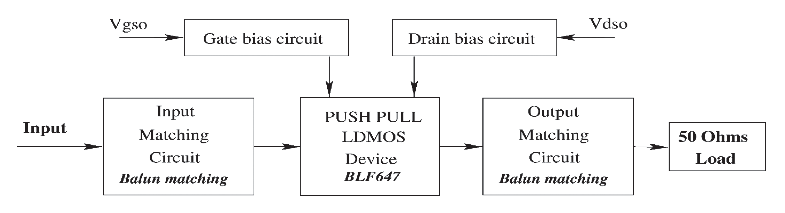
\includegraphics[width=3in]{Sample_Fig1.eps}\label{fig_first_case}}%
\hskip3pc
\subfloat[Case II]{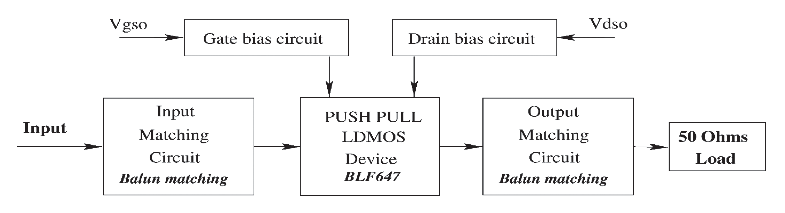
\includegraphics[width=3in]{Sample_Fig1.eps}\label{fig_second_case}}%
\caption[]{Sample sub figures in \LaTeX}
\label{fig_sim}
\end{figure*}


\section{Figures \& Tables}

The output for figures is:

\begin{figure}[!h]
%\centering\includegraphics[width=2.5in]{figurename.eps}
%%%call your figure name in the place "figurename.eps"
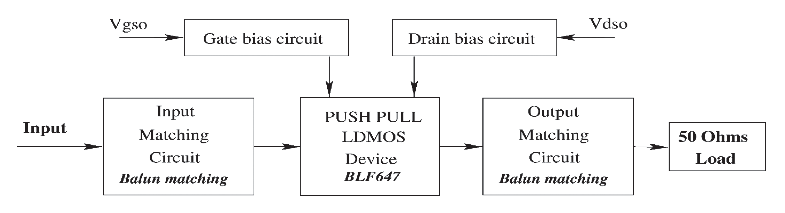
\includegraphics[width=3in]{Sample_Fig1.eps}
\caption{Insert figure caption here}
\label{fig_sim}
\end{figure}

 An example of a double column floating figure using two subfigures.
 (The subfig.sty package was already included in the class file.)
 The subfigure \verb+\label+ commands are set within each subfloat command, the
 \verb+\label+ for the overall figure must come after \verb+\caption+.
 \verb+\hfil+ must be used as a separator to get equal spacing.
 The subfigure.sty package works much the same way, except \verb+\subfigure+ is
 used instead of \verb+\subfloat+.


\vskip2pc

\noindent The output for tables is:

\begin{table}[!h]
\processtable{An Example of a Table\label{table_example}}%%%Table caption goes here
{\begin{tabular}{lllll}%%%The number of columns has to be defined here
\hline
\TCH{Head 1} & \TCH{Head 2} & \TCH{Head 3} & \TCH{Head 4} & \TCH{Head 5}\\
\hline
One & Two & Three & Four & Five\\ %%%% Table body
Six & Seven & Eight & Nine & Ten\\%%%% Table body
\hline
\end{tabular}}{}
\end{table}%%%End of the table

\section{Conclusion}
The conclusion text goes here.

\vfill\eject

%%%%%%%%%%% Please use the respective coding for Back matter section %%%%%%%%

\ack{Insert the Acknowledgment text here.}

\competing{Insert the Competing interests text here.}

\contribution{Insert the Contribution text here.}

\funding{Insert the Funding interests text here.}

\data{Insert the Data availability text here.}

\supplementary{Insert the supplementary text text here.}

%%%%%%%%% References %%%%%%%%%%%%%%%%%

\begin{thebibliography}{}

\bibitem[Arendt et~al.(2016)]{bib1}
\textbf{Arendt, D., Musser, J. M., Baker, C. V., Bergman, A., Cepko, C., Erwin, D. H.,
Pavlicev, M., Schlosser, G., Widder, S., Laubichler, M. D. et al.} (2016). The
origin and evolution of cell types. \textit{Nat. Rev. Genet}. 17, 744--757.

\bibitem[Ben-Tabou et~al.(2010)]{bib2}
\textbf{Ben-Tabou de-Leon, S. B. and Davidson, E. H.} (2010). Information processing at
the foxa node of the sea urchin endomesoderm specification network. \textit{Proc. Natl
Acad. Sci}. USA 107, 10103--10108.

\bibitem[Calestani and Rogers (2010)]{bib3}
\textbf{Calestani, C. and Rogers, D. J.} (2010). Cis-regulatory analysis of the sea urchin
pigment cell gene polyketide synthase. \textit{Dev. Biol.} 340, 249--255.

\bibitem[Cameron and Davidson (1991)]{bib4}
\textbf{Cameron, R. A. and Davidson, E. H.} (1991). Cell type specification during sea
urchin development. \textit{Trends Genet.} 7, 212--218.

\bibitem[Cameron et~al.(1987)]{bib5}
\textbf{Cameron, R. A., Hough-Evans, B. R., Britten, R. J. and Davidson, E. H.} (1987).
Lineage and fate of each blastomere of the eight-cell sea urchin embryo. \textit{Genes
Dev.} 1, 75--85.

\bibitem[Croce and McClay (2010)]{bib6}
\textbf{Croce, J. C. and McClay, D. R.} (2010). Dynamics of Delta/Notch signaling on
endomesoderm segregation in the sea urchin embryo. \textit{Development} 137, 83--91.

\end{thebibliography}

\end{document}
